\documentclass[a4paper,11pt]{article}

% 日本語対応
\usepackage{xeCJK}
\setCJKmainfont{Yu Gothic}

% 数学関連パッケージ
\usepackage{amsmath}
\usepackage{amssymb}
\usepackage{amsthm}
\usepackage{amsfonts}
\usepackage{mathtools}

% 図形描画用パッケージ
\usepackage{tikz}
\usepackage{pgfplots}
\pgfplotsset{compat=1.18}
\usetikzlibrary{intersections,patterns,angles,quotes,calc,fillbetween}

% その他パッケージ
\usepackage{graphicx}
\usepackage{enumitem}
\usepackage{float}
\usepackage{hyperref}
\usepackage{fancyhdr}
\usepackage{geometry}
\usepackage{xcolor}

% ページ設定
\geometry{
  a4paper,
  top=25mm,
  bottom=25mm,
  left=25mm,
  right=25mm
}

% 数式環境設定
\numberwithin{equation}{section}
\newtheorem{theorem}{定理}
\newtheorem{lemma}[theorem]{補題}
\newtheorem{proposition}[theorem]{命題}
\newtheorem{corollary}[theorem]{系}
\theoremstyle{definition}
\newtheorem{definition}[theorem]{定義}
\newtheorem{example}[theorem]{例}
\newtheorem{exercise}{問題}
\theoremstyle{remark}
\newtheorem*{remark}{注意}
\newtheorem*{solution}{解答}

% ヘッダーとフッターの設定
\pagestyle{fancy}
\fancyhf{}
\fancyhead[L]{数学問題}
\fancyhead[R]{\today}
\fancyfoot[C]{\thepage}
\renewcommand{\headrulewidth}{0.4pt}
\renewcommand{\footrulewidth}{0.4pt}

% タイトル情報
\title{数学問題}
\author{数学問題生成AIシステム}
\date{\today}

% ドキュメント開始
\begin{document}

\maketitle

% 問題セクション
\section*{問題}

% 問題文を挿入(変数で置換)
問題1の解答:

2次関数 $f(x) = 3x^2 - 12x + 11$ の頂点の座標を求めるには、まず頂点の公式を使用します。頂点の $x$ 座標は $x = -\frac{b}{2a}$ で与えられます。ここで、$a = 3$ 、$b = -12$ です。従って、

\[x = -\frac{-12}{2 \cdot 3} = 2\]

次に、この $x$ の値を $f(x)$ に代入して $y$ の値を求めます。

\[y = 3(2)^2 - 12(2) + 11 = 12 - 24 + 11 = -1\]

よって、頂点の座標は $(2, -1)$ です。

問題2の解答:

2次関数 $g(x) = x^2 - 4x + 3$ の $x$ 軸との交点を求めるには、$g(x) = 0$ と設定して $x$ の値を求めます。

\[x^2 - 4x + 3 = 0\]

この方程式を解くと、

\[x = \frac{4 \pm \sqrt{(-4)^2 - 4 \cdot 1 \cdot 3}}{2 \cdot 1} = \frac{4 \pm \sqrt{16 - 12}}{2} = \frac{4 \pm \sqrt{4}}{2} = \frac{4 \pm 2}{2}\]

従って、$x$ の値は

\[x = \frac{4 + 2}{2} = 3\] または \[x = \frac{4 - 2}{2} = 1\]

よって、$x$ 軸との交点は $(3, 0)$ と $(1, 0)$ です。

% 図形が必要な場合はここに挿入
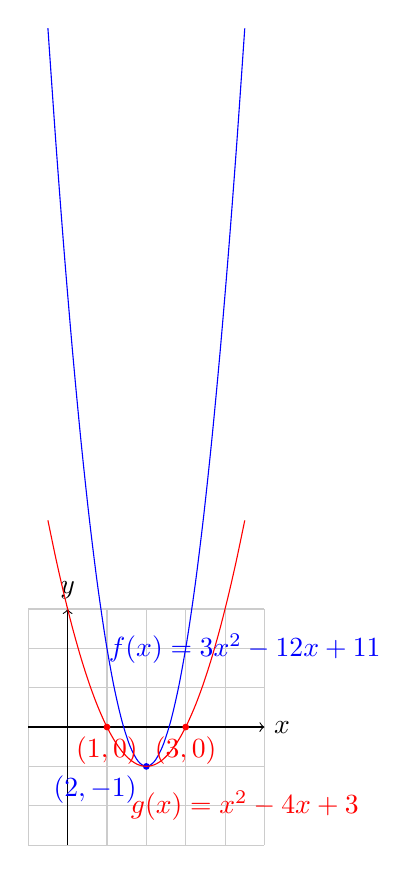
\begin{tikzpicture}[scale=0.5]
  % Draw axes
  \draw[thin,gray!40] (-1,-3) grid (5,3);
  \draw[->] (-1,0)--(5,0) node[right]{$x$};
  \draw[->] (0,-3)--(0,3) node[above]{$y$};

  % Draw function f(x) = 3x^2 - 12x + 11
  \draw[domain=-0.5:4.5,smooth,variable=\x,blue] plot ({\x},{3*\x*\x - 12*\x + 11});
  \filldraw[blue] (2,-1) circle (2pt) node[anchor=north east] {$(2,-1)$};

  % Draw function g(x) = x^2 - 4x + 3
  \draw[domain=-0.5:4.5,smooth,variable=\x,red] plot ({\x},{\x*\x - 4*\x + 3});
  \filldraw[red] (1,0) circle (2pt) node[anchor=north] {$(1,0)$};
  \filldraw[red] (3,0) circle (2pt) node[anchor=north] {$(3,0)$};

  % Labels
  \node[blue] at (4.5,2) {$f(x) = 3x^2 - 12x + 11$};
  \node[red] at (4.5,-2) {$g(x) = x^2 - 4x + 3$};
\end{tikzpicture}

% 解答セクション(オプショナル - 表示したくない場合はコメントアウト)
\section*{解答}

% 解答を挿入(変数で置換)
問題1の答え: $(2, -1)$, 問題2の答え: $x = 1$, $x = 3$

% 解説セクション(オプショナル - 表示したくない場合はコメントアウト)
\section*{解説}

% 解説を挿入(変数で置換)
問題1: 2次関数の頂点の座標は、公式 $\left(-\frac{b}{2a}, c - \frac{b^2}{4a}\right)$ を用いて求められる。ここで、$a = 3$、$b = -12$、$c = 11$ である。よって、頂点の$x$座標は $-\left(-12\right)/\left(2\cdot3\right) = 2$ であり、$y$座標は $11 - \left(-12\right)^2/\left(4\cdot3\right) = -1$ となる。したがって、頂点の座標は $(2, -1)$。

問題2: 2次関数 $g(x) = x^2 - 4x + 3$ の$x$軸との交点は、$g(x) = 0$ と置いて解くことにより求められる。$x^2 - 4x + 3 = 0$ を解くと、$(x - 1)(x - 3) = 0$ と因数分解できる。したがって、$x$軸との交点は $x = 1$ と $x = 3$ である。

\end{document} 